\documentclass[11pt,a4paper]{article}
\usepackage[utf8]{inputenc}
\usepackage[T1]{fontenc}
\usepackage{lmodern}
\usepackage{microtype}
\usepackage[margin=2.5cm]{geometry}
\usepackage{amsmath,amssymb}
\usepackage{graphicx}
\usepackage{caption}
\usepackage{subcaption}
\usepackage{booktabs}
\usepackage{xcolor}
\usepackage{hyperref}
\usepackage[capitalise]{cleveref}

\graphicspath{{images/}}

\title{A Sample Article with Figures and Tables}
\author{Your Name\\\small Your Institution}
\date{\today}

\begin{document}
\maketitle

\begin{abstract}
This template shows how to include images, arrange subfigures, typeset
tables with \texttt{booktabs}, number equations, and reference all of them
with \texttt{cleveref}. Double-click anywhere in the PDF to jump to the
matching line in the source.
\end{abstract}

\section{Including images}
Images live in the \texttt{images/} folder. Upload your own by dragging files
onto the file tree, or paste an image straight into the editor.
\Cref{fig:landscape} is a single figure, and \cref{fig:pair} shows two
images side by side.

\begin{figure}[htbp]
  \centering
  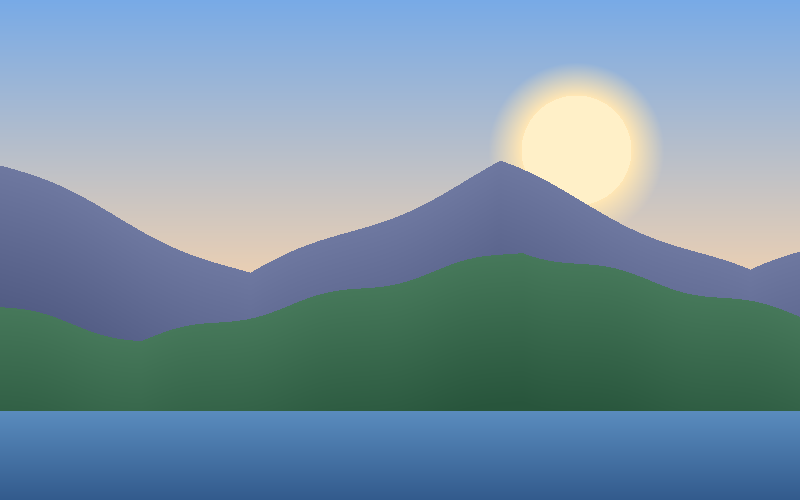
\includegraphics[width=0.7\linewidth]{landscape.png}
  \caption{A landscape, included with \texttt{\textbackslash includegraphics}.}
  \label{fig:landscape}
\end{figure}

\begin{figure}[htbp]
  \centering
  \begin{subfigure}[b]{0.45\linewidth}
    \centering
    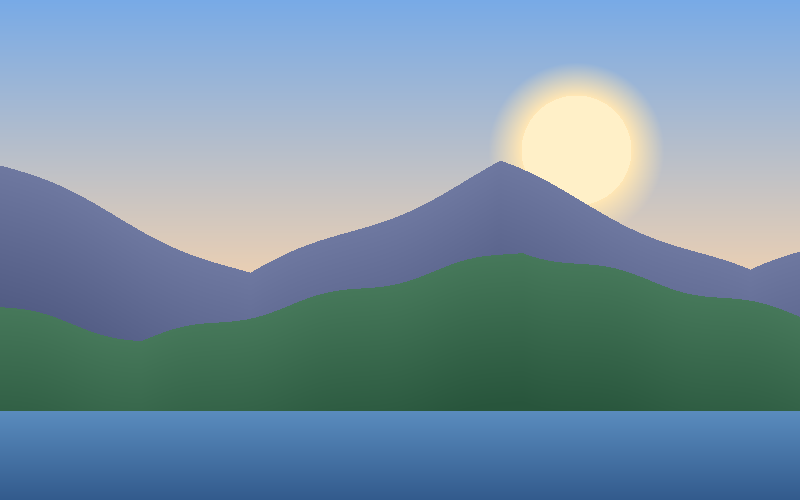
\includegraphics[width=\linewidth]{landscape.png}
    \caption{First image}
    \label{fig:pair-a}
  \end{subfigure}\hfill
  \begin{subfigure}[b]{0.45\linewidth}
    \centering
    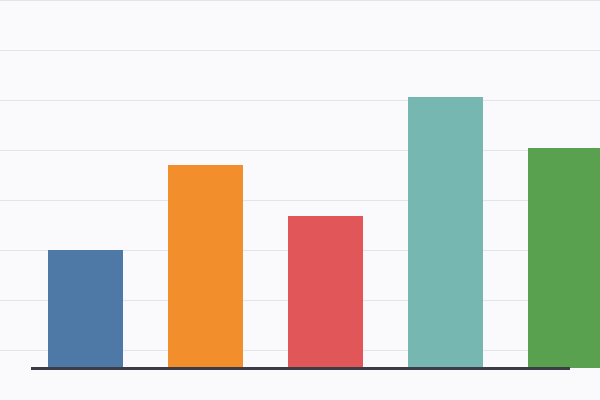
\includegraphics[width=\linewidth]{chart.png}
    \caption{Second image}
    \label{fig:pair-b}
  \end{subfigure}
  \caption{Two subfigures: \subref{fig:pair-a} and \subref{fig:pair-b}.}
  \label{fig:pair}
\end{figure}

\section{Tables}
\Cref{tab:results} uses \texttt{booktabs} rules for a clean look.

\begin{table}[htbp]
  \centering
  \caption{Results of an imaginary experiment.}
  \label{tab:results}
  \begin{tabular}{lrrr}
    \toprule
    Method & Accuracy (\%) & Time (s) & Memory (MB) \\
    \midrule
    Baseline   & 81.2 & 12.4 & 512 \\
    Improved   & 87.9 & 10.1 & 498 \\
    \textbf{Ours} & \textbf{92.3} & \textbf{8.7} & \textbf{430} \\
    \bottomrule
  \end{tabular}
\end{table}

\section{Mathematics}
The Gaussian integral, \cref{eq:gauss}, is a classic:
\begin{equation}
  \int_{-\infty}^{\infty} e^{-x^2}\,\mathrm{d}x = \sqrt{\pi}.
  \label{eq:gauss}
\end{equation}
Aligned equations work too:
\begin{align}
  (a+b)^2 &= a^2 + 2ab + b^2, \label{eq:binom1}\\
  (a-b)^2 &= a^2 - 2ab + b^2. \label{eq:binom2}
\end{align}

\section{Lists}
\begin{itemize}
  \item Bullet lists with \texttt{itemize}
  \item Numbered lists with \texttt{enumerate}
  \item \textcolor{blue!60!black}{Coloured text} with \texttt{xcolor}
\end{itemize}

\end{document}
